%\documentclass[11pt, oneside]{book}
\documentclass[11pt, twoside]{book}  %importante cambiar si es libro
\usepackage[utf8]{inputenc}
\usepackage[T1]{fontenc}

%%%%%%%%%%%%%%%%%%%%%%%%%%%%%%%%%%%%%%%%%%%%%%%%%%%%%%%%%
%   Paquetes y librerías iniciales para un documento,   
%           Graficos, simbolos, tablas, bibliografía
%%%%%%%%%%%%%%%%%%%%%%%%%%%%%%%%%%%%%%%%%%%%%%%%%%%%%%%%%
%---------------------------------------------------------------------------
% Esto es para que el LaTeX sepa que el texto está en español:
\usepackage[spanish,es-noshorthands,es-tabla]{babel}
\selectlanguage{spanish}
%---------------------------------------------------------------------------
% para uso en modo matemático
\usepackage{amssymb}
\usepackage{amsthm}
\usepackage{amsmath}

%---------------------------------------------------------------------------
% Para las imagenes 

\usepackage[dvips]{graphicx}
\graphicspath{{Figuras/}} % se fija el camino para las figuras
\usepackage{rotating}  %para poder rotar las figuras
\usepackage{wrapfig}

%---------------------------------------------------------------------------
% PIES DE FOTOS Y TABLAS 

\usepackage{float} % para objetos flotantes
\usepackage{caption} % para los pies de fotos o tablas
\usepackage{subcaption}
\captionsetup{font=small,labelfont=bf} % para tamaño y tipo fuentes pie de foto
\usepackage{multirow} % para las tablas unir columnas
\usepackage{multicol} %para escribir en multiples columnas

% Referencias y biblio

\usepackage{pdfpages}
%\usepackage[pdftex,breaklinks=true,hidelinks]{hyperref} % para referencias/indice en pdf

\usepackage[
breaklinks=true,colorlinks=true,
linkcolor=blue,urlcolor=blue,citecolor=blue,% PDF VIEW
linkcolor=black,urlcolor=black,citecolor=black,% PRINT
bookmarks=true,bookmarksopenlevel=2]{hyperref}

\usepackage{emptypage}
\usepackage{ragged2e} %Justificacion

%\usepackage[toc,title,page]{appendix}

%Para bibliografía
\usepackage[numbers,square]{natbib}
%\bibliographystyle{apalike}
\bibliographystyle{IEEEtran}

%%%%%%%%% Habituales estilos
%plainnat
%%abbrvnat
%unsrtnat  %Items in bibliography sorted in order cited)
%IEEEtran

%

%%%%%%%%%%%%%%%%%%%% Formato de la UAL %%%%%%%%%%%%%%%%%%%%%%%%%%%%%%%%%


%\usepackage{UAL}
\usepackage[print,doble]{UAL}
\usepackage{codigo}

%%%%%% PAQUETES INCORPORADOS POR EL USUARIO

\usepackage{longtable}   %Tablas largas
\usepackage{verbatim}
\usepackage{textcomp} %para completar los signos válidos
\usepackage{eurosym} %símbolo del euro [\euro]
\usepackage[bottom]{footmisc}



%%%%%%%%%%%%%%%%%%%%%%%%%%%%%%%%%%%%%%%%%%%%%%%%%%%
% Datos identificativos del TFG                   %
%%%%%%%%%%%%%%%%%%%%%%%%%%%%%%%%%%%%%%%%%%%%%%%%%%%

\author{Faccion de Osadia}
\titulo{Libro de estilo para la  memoria del TFG de informática de la UAL }
\subTitulo{DEPARTAMENTO DE
INFORMÁTICA\\  ÁREA DE LENGUAJES Y SISTEMAS INFORMÁTICOS}
\estudios{Grado en Informática }
\universidad{UNIVERSIDAD DE ALMERÍA}
\director{Isabel Maria del} 
\direct{Aguila Cano}
\curso {2020/2021}


\pagestyle{cab}

\begin{document}
\frontmatter

\portada

\begin{dedicatoria}
    Texto de la dedicatoria
\end{dedicatoria}


%%%%%%%%%%%%%%%%%%%%%%%%%%%%%%%%%%%%%%%%%%%%%%%%%%%%%%%%%%%%%%%%%%%%%%%%%%%%
%%%%%%%%%%%%%%% ESTO ES PARA LA TABLA DE CONTENIDOS (INDICE)%%%%%%%%%%%%%%%%


\setcounter{secnumdepth}{3} %niveles en capitulos hasta (1.1.1)
\setcounter{tocdepth}{3} %niveles en indice hasta (1.1)


\addtocontents{toc}{~\hfill\small{Página}\par} %añade "pagina" a tabla de contanidos
\addtocontents{toc}{\vspace{2pt} \hrule \vspace{5mm} \par}

%\renewcommand\contentsname{Índice de contenidos}
\tableofcontents
\listoffigures % indice de figuras
\listoftables % indice de tablas
\lstlistoflistings % indice de listados


%---------------------------------------------------------------------------
% comienzo de relacion abreviaturas y/o acrónimos
%---------------------------------------------------------------------------


%\addcontentsline{toc}{section}{ABREVIATURAS}
\clearpage
\vspace{0.2cm}
\section*{ABREVIATURAS}

\begin{tabular}{ l   |    l  }
	

&\\
   ESI & Escuela Superior de ingeniería \\
   InSo & Ingeniería del Software \\
    SBSE& Search based software engineering\\
   TFG & Trabajo fin de grado\\
   
      UAL & Universidad de Almería \\
      &\\

\end{tabular}


%\addcontentsline{toc}{section}{ABREVIATURAS}



% Borra el bloque si sólo queremos resumen en contraportada
\addcontentsline{toc}{chapter}{Resumen y Abstract}

\chapter*{Resumen y Abstract}

En este archivo se incluirá tanto el resumen en castellano como su traducción al inglés. Los dos párrafos estarán ligeramente separados.

El  propósito  del  trabajo  en  una  o  dos  frases.  El  diseño  y metodología  utilizada,  los  resultados  más  significativos  del trabajo realizado y un breve resumen de las conclusiones. Debe ser conciso y presentar los resultados obtenidos tras la ejecución del TFG. 

\vspace{1.5cm}

%\section*{Abstract}
Put here  the english tranlation  ... . Debe ser conciso y presentar los resultados obtenidos tras la ejecución del TFG. Los dos parrafos estarán ligeramente separados.


%se suelen utilizar archivos separados, por capitulos para agilizar la compilación en las versiones intermedias
\mainmatter
\marcagua


\chapter {Introducción}
\label{sec:intro}


En este documento se va a realizar una plantilla que mostrará tanto el formato como el posible contenido de un Trabajo fin de estudios modelo, para los estudios de informática de la Universidad del Almería.
Servirá de  ayuda  para  la  realización  de  los trabajos  académicos  que,  durante  la  formación  universitaria,  constituyen  una  actividad  permanente.

El trabajo académico requiere precisión y rigor conceptual, dominio de fuentes de información y capacidad de argumentación teórica.  No es un  resumen de las ideas de otras personas, sino una disertación sobre un tema, tomando como referencia  la información  que existe sobre el  mismo en diversas fuentes. Recuerda copiar de uno es un plagio, copiar de muchos investigación. \cite{malaga}

Esta  plantilla está escrita en \LaTeX.
El \LaTeX (escrito LaTeX en texto plano) es un sistema de composición de textos, orientado a la creación de documentos escritos que presenten una alta calidad tipográfica. Por sus características y posibilidades, es usado de forma especialmente intensa en la generación de artículos y libros científicos que incluyen, entre otros elementos, expresiones matemáticas. \cite{wiki}

LaTeX está formado por un gran conjunto de macros de TeX con la intención de facilitar el uso del lenguaje de composición tipográfica,  \LaTeX, creado por Donald Knuth. Es muy utilizado para la composición de artículos académicos, tesis y libros técnicos, dado que la calidad tipográfica de los documentos. 

Este lenguaje presupone una filosofía de trabajo diferente a la de los procesadores de texto habituales (conocidos como WYSIWYG, es decir, <<lo que ves es lo que obtienes>>) y se basa en instrucciones. Tradicionalmente, este aspecto se ha considerado una desventaja (probablemente la única). Sin embargo, LaTeX, a diferencia de los procesadores de texto de tipo WYSIWYG, permite a quien escribe un documento centrarse exclusivamente en el contenido, sin tener que preocuparse de los detalles del formato. Además de sus capacidades gráficas para representar ecuaciones, fórmulas complicadas, notación científica e incluso musical, permite estructurar fácilmente el documento (con capítulos, secciones, notas, bibliografía, índices analíticos, etc.), lo cual brinda comodidad y lo hace útil para artículos académicos y libros técnicos.

Para la elaboración de esta guía además de la experiencia de su autora se ha utilizado como referencia las normas sobre Trabajos fin de Grado (TFG) y Trabajos Fin de Master (TFM) del diversas Universidades, entre ellas la Universidad de Málaga \cite{malaga} y la Universidad de Alicante \cite{alicante}


\chapter{Consideraciones generales} 
\label{sec:consideraciones}


La lista de consideraciones puede ser amplia, pero hay unos requisitos clave que se tienen que verificar.
El  escrito  tiene  un  carácter  formal,  de  ahí  que  no  se  puede  desarrollar  un  discurso  humorístico;  tampoco  recurrir  al  sarcasmo  y  al  empleo  de  un  vocabulario  coloquial.  El  lenguaje que se utilice ha de ser técnico, riguroso, analítico y preciso. 

Aunque recoge el trabajo personal no se debe utilizar la  primera  persona  del  singular:  “yo...”; la fórmula que se ha de utilizar en la disertación es el impersonal: “se plantea...”, “la  tesis  de  la  que  se  parte...”  (y  no  “parto  de  la  tesis...”).  De  este  modo,  el  estilo  académico   utilizado   se   caracteriza   por   formas   verbales   pasivas,   pronombres   y   construcciones impersonales y vocabulario específico. En algunas ocasiones y por deformación del uso del inglés se puede utilizar la primera persona del plural, aunque en TFG/TFM no es recomendable, salvo que se describan trabajos específicos realizados en equipo.

Es de vital importancia el uso correcto del lenguaje (ortografía, expresión, signos de puntuación).  Si es necesario se deben consultar diccionarios generales o específicos para aclarar significados de términos así como para el empleo de sinónimos y antónimos. 

El  objetivo  fundamental  del  escrito  es  demostrar  los  propios  conocimientos  sobre  la  materia de la manera más completa posible. Es importante dar respuesta  a las  premisas,  las  preguntas  o  las  cuestiones  de  investigación  o  indagación  que  se  hayan  establecido como punto de partida y que tendrán que ser coherentes con los objetivos del trabajo.

La forma es tan importante como el fondo. Es importante la coherencia del formato en especial en la bibliografía. Queda fuera de esta guía tratar sobre como realizar las citas y los distintos tipos de bibliografía. La biblioteca de la universidad ofrece cursos y asesoramiento para quienes lo necesiten. Cabe descartan, que cada disciplina utiliza distintos tipos de normas para la realización de las citas.

En líneas generales, el trabajo académico consta de cuatro partes importantes: la introducción, el desarrollo, las conclusiones y las referencias bibliográficas. A estas cuatro se le añade una quinta relativa  a  los  anexos  (información  complementaria  y/o  aclaratoria), aunque los trataremos con detalle en el capítulo \ref{sec:apartados}.  Es  importante  conocer  que  la  estructura de la memoria no  es  la  que  se  sigue  secuencialmente cuando  una  persona  se  plantea escribir el documento. Por  ejemplo,  la  introducción,  que  es  la  primera  parte  de  todo  trabajo,  es  la  última que se elabora.

Cuando  una  persona  se  enfrenta  a  este  tipo  de  trabajos no obtiene una memoria “a la primera” ni “de una sola vez”. Antes de llegar al texto definitivo, éste debe haber pasado por varios borradores y numerosos cambios y reordenaciones.

Puesto que es necesaria una colaboración estrecha entre alumnos y tutores del trabajo, buscar entornos de edición colaborativa puede se una buena solución. La mejor recomendación es \url{https://www.overleaf.com} que además de numerosas plantillas ofrece una ayuda inestimable sobre el lenguaje \LaTeX{}, que si bien no es profunda, si se tocan brevemente todos los temas.

\chapter{Normas fundamentales del formato} 
\label{sec:funda}

La memoria del Trabajo Fin de Grado/Máster se presentará en formato  UNE  A4,  salvo  que  las  características  especiales  del  trabajo  presentado  no  lo permitieran.

\section {Estilo,  Tipografía y    Maquetado}

Se podrán utilizar las siguientes familias de tipos de letras \url{https://tug.org/FontCatalogue/}, no se recomiendan tipos de letras con decoración excesiva:

	\begin{center}
	\begin{tabular}{p{2cm}p{7.5cm}c}
		\textbf{Tipo} & \textbf{Fuente} & \textbf{Anchura} \\ \hline
         Familia 1 & Arial, Helvética, Tahoma  	\ldots & Variable \\
         Familia 2 & Times New Roman, Palatino  Linotype,  	\ldots & Variable  \\
         Familia 3 & Courier  New,  Miriam Fixed \ldots & Fija\\
         \hline
	\end{tabular}
	\end{center}



\begin{table} 
	\begin{center}
	\begin{tabular}{l c c}
		\textbf{Tipo} & \textbf{Fuente} & \textbf{Anchura} \\ \hline
         Familia 1 & Arial, Helvética, Tahoma  	\ldots & Variable \\
         Familia 2 & Times New Roman, Palatino  Linotype,  	\ldots & Variable  \\
         Familia 3 & Courier  New,  Miriam Fixed \ldots & Fija \\
         \hline
	\end{tabular}
	\end{center}

	\caption{\label{tab:letras}Tipos de letras.}
\end{table}


La familia 1 se recomienda para los títulos de las distintas secciones del documento.

La familia 2 se recomienda para los párrafos normales.

La familia 3 se recomienda para escribir, por ejemplo, porciones de código, debido a su tamaño fijo donde es necesario un texto tabulado y se alinee perfectamente, así como cualquier otro uso de texto de tamaño de letra fijo.

Se recomienda el uso del tipo de letra Palatino Linotype en itálica para la escritura de fórmulas sencillas, para aquellas que sean más complejas se podrá usar un editor de ecuaciones, ejemplos:

$ x^2+y^2=r^2,    a+b=c$

Si fuese necesario se puede utilizar un entorno ecuación para después poder referenciarlo en el texto. La ecuacion  \ref{ec:ecuacion} es un ejemplo, pero se convierte en un flotante como las tablas y las figuras. La potencia de \LaTeX{} para la edición de ecuaciones supera el alcance de este documento, se sugiere consultar otras fuentes para ampliar la información sobre su uso.

\begin{equation}
\label{ec:ecuacion}
    x_1= \frac{-b+\sqrt{b^2-4*a*c}}{2*a}
\end{equation}




Las dimensiones del la zona de texto se definen a través del \emph{geometry}, \lstinline[language=enparrafo]!geometry!, un paquete de latex que en este caso se incluye en el estilo \textbf{UAL}, \lstinline[language=enparrafo]!\usepackage{UAL}!.

\section {Estilo ual de latex}

En el estilo se define la portada y contraportada según las recomendaciones de la escuela superior de ingeniería, véase la figura \ref{fig:facultad}.

\begin{figure}
	\begin{center}
		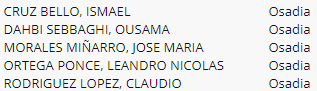
\includegraphics[width = 0.5\textwidth]{Capturas/Equipo.PNG}
	\end{center}
	\caption{\label{fig:facultad} Logotipo de la Escuela Superior de ingeniería }
\end{figure}



El estilo generado permite definir un documento a una cara o doble cara para lo que se tiene que seleccionar la opción "print" al incluir el paquete estilo (\lstinline[language=enparrafo]!\usepackage[print]{UAL}!). De esta forma se podrá personalizar, el pasar al la página impar en cada sección o bien a la páginas siguiente. %Para lo que se ha personalizado el comando $\ $siguiente que se ha de colocar antes del inicio de cada sección.
Además se fija la marca de agua. Otras cuestiones incorporados en el estilo son los distintos tipos de cabeceras y pies de página necesarios.

Un aspecto importante son los elementos flotantes de latex, en especial tablas y figuras. Estos son los elementos que después pueden incorporarse en los índices de la cabecera del documento. En los casos que se utilicen "códigos" también se puede incluir un índice de listados, \lstinline[language=enparrafo]!\usepackage{listing}!.

Si es necesario se puede trabajar con los paquetes para tablas largas o con aquellos que permiten hacer subfiguras.

 \section{Figuras y tablas}

Las  figuras  (o  gráficos)  y  tablas  (cuadros)  que  se  incorporen  deben  ir  numerados  (números  arábigos)  y  tener  un  título,  y  siempre  tendrán  que  tener  relación  con el contenido expuesto.  Todo elemento flotante debe referenciarse en el texto y debe colocarse  preferiblemente después de la primera vez que se cita en el texto.

Las  gráficas, fotografías,  los  diagramas,  mapas,  dibujos,  etc.serán  considerados como  figuras. Es importante que se incluya el origen de la figura, en la etiqueta, si la ha hecho el autor se coloca el texto "elaboración propia".

No se deben poner gráficos, figuras y fotos sólo para rellenar siempre se nota demasiado. Los gráficos y figuras deben ir referenciados en el texto, sino es mejor no incorporarlas en la memoria.



 \section{Listados de código}

En el dominio de la informática es habitual que un TFG/TFM deba incluir porciones de código fomateado. Incluso que se definan como un un elemento flotante especial. En \LaTeX{} existen muchas formas de resolver esta cuestión. Se ha definido un estilo llamado \lstinline[language=enparrafo]!codigo.sty! que implementa un ejemplo. Los archivos de código están una carpeta aparte igual que las figuras. \footnote{Se puede sincronizar con repositorios de código tipo \url{www.github.com} se emplea overleaf, pero es necesario mantener dos proyectos}

\subsection{Utilización del entorno verbatim}
Lo que en latex se coloca dentro de un entorno verbatim deja de ser código latex y se representan tal como aparece. Pero suele tener interacciones con el paquete  gráfico tikz. por lo que no es recomendable, es mejor usar \lstinline[language=enparrafo]!\lstinline!

\begin{verbatim}
#include <stdio.h>

int main()
{
        printf("Hola mundo");
        return 0;
}
\end{verbatim}

\subsection{Utilización de paquete listing}


Se puede escribir directamente el código dentro de un entorno y si no se especifica nada se utilizan los parámetros por defecto. Para detalle de como configurar esta utilidad es conveniente revisar la documentación del paquete

\begin{lstlisting}[caption=Ejemplo ]
#include <stdio.h>

int main()
{
        printf("Hola mundo");
        return 0;
}
}
\end{lstlisting}


Ejemplo de inclusión sin utilizar un objeto flotante. No aparecerá en el índice por poner \lstinline[language=enparrafo]!nolol=true!.

\lstinputlisting[firstline=1, firstnumber=1, nolol=true]{holamundo.c}


\lstinputlisting[caption=,language=pseudo, caption=Ejemplo en pseudocodigo]{holamundo.psc}


Realmente se trata de un paquete muy complejo que se puede complementar con el uso de entornos personalizados, cuya explotación exhaustiva queda fuera de este libro de estilo.


\chapter {Buenas prácticas}


En esta sección se incluyen una serie de cuestiones o buenas prácticas que se derivan de la experiencia, de normas básicas de elaboración de textos científicos \cite{alba2009}, y de las normas gramaticales básicas.

\begin{enumerate}
    \item Cuidado con el espacio entre palabras, utilizar \emph{hyphenation} para cortar o no palabras con los guiones. Aunque por defecto el paquete de español de latex lo gestiona aceptablemente bien.

\item Los signos de puntuación (comas, puntos, puntos y comas, dos puntos) así   como   el   cierre  de   comillas, paréntesis e   interrogaciones han   de   ir inmediatamente   a   continuación   (sin   espacios)   de   la   palabra   anterior   y separados  por  un  espacio  de  la  palabra siguiente.  De  modo  contrario,  los signos   de   apertura   de   comillas, paréntesis e   interrogaciones deben   ir separados  por  un  espacio  de  la  palabra  anterior e inmediatamente  antes  (sin espacio) de la palabra posterior.


\item En las listas \lstinline[language=enparrafo]!\begin{itemize}! \lstinline[language=enparrafo]!end{itemize}! o enumeraciones \lstinline[language=enparrafo]!\begin{enumerate}! donde no aparezca un verbo, es decir no se a una oración completa no se pone punto al final. Sólo se pone punto en el último item de la lista para finalizar el párrafo.

\item Por la misma razón no se deben acabar los títulos y los subtitulos con un punto. En los pies de figuras y tablas queda a criterio del autor y tutor, pero la recomendación es no ponerlo.

\item Aunque en español las siglas puedan marcarse con puntos entre letra y letra,  se  recomienda  utilizarlas  siempre  en  mayúscula  (siempre  sin  tilde) y  sin los    puntos.  

\item La  primera  vez  se emplea una acrónimo debe  ser  definido, incluyendo   el   texto   de   la   definición   entre   paréntesis   y   marcando   con mayúsculas  las  letras  que  dan  lugar  al  acrónimo.  Ejemplo:  MCU  (Multipoint Control  Unit).  En  subsiguientes  apariciones  del  acrónimo  no  debe  volverse  a incluir  la  definición.  Se  recomienda  adjuntar  al  principio  del  proyecto  una relación    detallada    de    los    acrónimos    y    su    significado,    ordenados alfabéticamente.


\item Existen tres tipos de comillas: las españolas o latinas (<<comillas >>), las inglesas ("comillas") y las simples ('comillas' ). Use un único tipo a lo largo del texto. En escritos científicos es más común encontrar las inglesas o las simples. Empléelas siempre que efectúe citas textuales extraídas de algún documento.  También están las comillas abiertas y cerradas ``comillas ''. 


\item Evite   emplear   innecesariamente   palabras   o   expresiones   en   inglés cuando  en  español  exista  un  equivalente.  El  uso  de  términos  ingleses  no aceptados debe circunscribirse al campo técnico. Por ejemplo "planning del proyecto" en lugar de "planificación del proyecto". 

\item No se deben traducir sin comprobar la validez términos técnicos muy específicos si dichas traducciones no se encuentran más o menos asumidas por la comunidad científica (es decir, las   ha   leído   o   escuchado   repetidas   veces).   En   el   texto   los   términos   y expresiones inglesas no aceptados deben aparecer en cursiva.

\item Cuando  se  referencien  símbolos  matemáticos  en  el  texto,  estos  han  de aparecer   en   cursiva   y   de   la   misma   manera   a   como   aparecen   en   las ecuaciones.

\item No se deben usar frases con el verbo principal en infinitivo y sin articular. Por ejemplo no se debe escribir  “En  primer  lugar,  destacar  que  los  resultados  se  obtuvieron  por simulación”. En su lugar  “En primer  lugar se ha  de  reseñar que  los resultados...” (o “se debe”, “es preciso”, “hemos de”, “cabe” reseñar).

\item El sujeto (salvo que se intercale una frase subordinada) no se puede separar por comas del predicado. 

\item Se ha de ser   coherente  con  el  uso  de  los  tiempos  verbales.  Si  describe  lo  que  se  ha hecho en pasado, se ha de continuar  con ese tiempo a lo largo de la memoria. 

\item No se debe abusar del  anidamiento  de oraciones  subordinadas.  En  su  lugar  es recomendable  usar  una  secuencia  de  oraciones  cortas,  que  son  de  más  fácil compresión. Asimismo, se deben evitar las negaciones encadenadas 
“no  aumentar  el  parámetro  beta  implica  que  no  se  aumenta  la  ganancia”, siendo preferible afirmar “reducir el parámetro beta reduce la ganancia”.

\item Se han de reescribir   las  formas pasivas.  Utilice,  en  su  lugar,  la  pasiva  refleja.  Es preferible “se ha desarrollado un sistema” a “un sistema ha sido desarrollado”. La construcción en pasiva es típicamente inglesa y su abuso denota que estás traduciendo algo (lo cual no es pecado si dices de quien lo traduces). Lo mejor es escribir en castellano. Ejemplo: “Puede  que  sean  retrasadas...”    se  debería  escribir  “Pueden  retrasarse”  o  “puede  que  se retrasen”.

\item Todos los párrafos concluyen con un punto final.

\item En  el  texto,  si se utilizan números se han de expresar   con  palabras   si  son  menores  o  iguales  que veinte y con números si son superiores a ese valor o presentan decimales.

\item A  la  hora  de  emplear  la  coma  o  el  punto  para  expresar  los decimales en los números se debe ser congruente, no usarlos indistintamente.

\item  Los términos  (adjetivos  y  adverbios)  valorativos  que  resulten  exagerados  o poco científicos deben evitarse. Por ejemplo,  “notablemente” o “sustancialmente” antes que “espectacularmente”, “enormemente”, “aplastantemente”, “drásticamente”o “fenomenalmente”. Al hablar de un resultado  o  de  un  producto  de  Ingeniería, es preferible “de forma adecuada o muy conveniente” antes que “perfectamente”.

\item En un texto científico es preferible, para concluir una relación que se sabe que es muy larga, emplear “etc.” que los puntos suspensivos (“...”).

\item El  vocabulario debe ser rico y no repetir términos dentro de la misma frase o  párrafo.  Por  ejemplo,  para comentar  lo  que  una  figura  enseña,  puede  decir “en  la  figura  se  muestra,  se  refleja,  se  indica,  se  ilustra,  se  presenta,  se observa, se detecta, se comprueba, se contempla, se evidencia, se confirma,...”

\item Las  frases han de concordar en  sujeto y predicado.

\item  El término “demostrar” es muy riguroso (salvo  que  exista  una  auténtica demostración). Una figura muestra pero no suele demostrar nada. 

\item Salvo en casos muy puntuales (citas textuales, por ejemplo), detrás de los dos puntos (“:”) se sigue en minúsculas.

\item No se debe utilizar la palabra \emph{optimizar} en vano.

\item Escribir  un  trabajo  de  investigación,  no  es  hacer  literatura  barroca.  Cada  frase  y  cada  palabra debe servir para algo. Si no limitamos nuestra verborrea, nos podemos meter en un lío.

\item Si  se  va  a  hacer  una  descripción  de,  por  ejemplo,  siete  etapas  de  algo,  no  está  de  más, primero listarlas y luego iniciar la descripción.



\end{enumerate}

 Otra lista de errores y/o consideraciones se muestra en la figura \ref{fig:errores}.
 
\begin{figure}[h]
	\begin{center}
		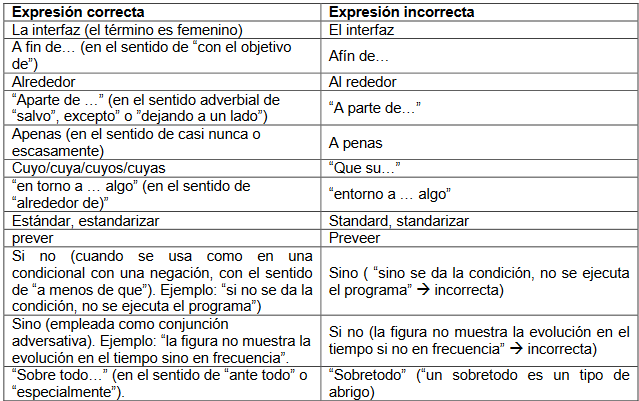
\includegraphics[width = 0.95\textwidth]{Figuras/errores}
	\end{center}
	\caption{\label{fig:errores} Errores habituales}
\end{figure}



 
 \chapter{Apartados del trabajo }
\label{sec:apartados}

Tal como se indicó en la sección \ref{sec:intro}, además de la portada y datos de identificación, los apartados de referencia el trabajo tendrán cuatro partes diferenciadas (introducción, desarrollo, conclusiones y  referencias bibliográficas) y los anexos.

 \section{Bloque inicial de identificación}

 \subsection{Portada y contraportada}  
La portada es la presentación del trabajo en la que se ha de indicar el título y subtítulo (si  lo  hubiera),  el  autor  o  la  autora  del  mismo,  el  nombre  del  tutor  o  de  la  tutora,  el  Grado  que  cursa, la institución y el año. Su formato está fijado por la ESI.


\paragraph{Titulo}

Debe describir el contenido del trabajo, 10 o 15 palabras. Un buen título nos servirá para identificar el objetivo principal del estudio.

\paragraph{Resumen }
Debe contener:
\begin{itemize}
    \item El  propósito  del  trabajo  en  una  o  dos  frases
    \item El  diseño  y metodología  utilizada
    \item Los  resultados  más  significativos  del trabajo realizado 
    \item Un breve resumen de las conclusiones.
\end{itemize}


 \subsection{Portadilla}
A decisión del autor del trabajo se puede incorporar una dedicatoria, y también una copia del resumen de la contraportada. En el caso de no encuadernarse el trabajo \footnote{se ha seleccionado la opción \emph{print} al incorporar el estilo y \emph{twoside} al seleccionar la clase latex del documento}, es recomendable incorporar el resumen en esta portadilla.

También se puede añadir una  sección  de  agradecimientos  (evidentemente  no  obligatoria)  define  un apartado  donde  el autor  puede  (y  quizás  debe)  referenciar  a  aquellas  personas  y/o  instituciones  que,  de  manera generosa, han colaborado de algún modo en la gestación y desarrollo del TFG/TFM.
Igualmente el autor también  puede  utilizar  este  apartado libremente  para mencionar  a  aquellos  familiares,  compañeros, amigos, etc., de los que ha recibido apoyo personal, moral o afectivo. 

 \subsection{Índices y listas}

Cada índice puede o no  comenzar en una nueva página (utilizando el comando  \lstinline[language=enparrafo]!\clearpage! , se incluirán los índices que se estimen necesarios, en este orden:

\begin{itemize}
    \item Índice de contenidos: (obligatorio  siempre)  se  incluirá  un  índice  de  las secciones  de  las  que  se  componga  el  documento,  la  numeración  de las divisiones  y  subdivisiones  utilizarán  cifras  arábigas y harán mención a la página del documento donde se ubiquen.
    
\item Índice de figuras: si el documento incluye figuras se podrá incluir también un índice con su relación, indicando la página donde se ubiquen.

\item Índice de tablas: en caso de existir en el texto, ídem que el anterior.

\item Índice de listados: en caso de existir en el texto, ídem que el anterior.

\item Índice de abreviaturas, siglas, símbolos,etc.:en  caso  de  ser  necesarios  se podrá incluir cada uno de ellos.

\end{itemize}

 \section{Introducción}
Se hará énfasis a la importancia de la temática, su vigencia y  actualidad;  se  planteará  el  problema  a  investigar,  así  como  el  propósito  o finalidad de la investigación. En cuanto a incluir o no un anticipo de las conclusiones habitualmente depende del tipo de trabajo y suele estar a criterio de tutor.

Cabe destacar la necesidad de incorporar los objetivos si no se utiliza un apartado específico para ello.

 \section{Desarrollo o cuerpo del documento}
Incluye   el  desarrollo  de  los  aspectos  esenciales  del  tema.  Aquí  se  evidenciará la capacidad de organización y estructuración de los argumentos de quien escribe. Se han de evitar las contradicciones y asegurar la coherencia entre las ideas expresadas. El desarrollo se  basa  en  la  exposición,  en  el  análisis  reflexivo  y  en  el  contraste  de  ideas.  En  este  proceso  argumentativo,  las  ideas  principales  y  secundarias  deben  ir  acompañadas  de  \textbf{citas  de  fuentes  bibliográficas} y de ejemplos que lograrán sustentar la tesis principal del trabajo. 
%%%%%%%%%%%%%%%%%%%%%%%%%%%%%%%%

Los objetivos del trabajo o bien se han definido en la introducción o se describen como primer apartado del cuerpo del documento.

En informática en la Universidad de Almería (UAL) si bien todos los trabajos son monográficos, también cierto que la mayor parte de ellos tienen una componente puramente técnica de desarrollo de aplicaciones software, donde se aplica alguna metodología de desarrollo de software \cite{SWEBOK2014}. El apartado desarrollo deberá balancear la componente  técnica con la de investigación propia de un trabajo monográfico.

En el aspecto mas investigador,  es  importante  destacar  dos  aspectos \cite{alicante}:  
\begin{itemize}
    \item [Primera]  Es  muy  importante  la  relectura  de  las  fuentes. No basta con   resumir   lo  leído  sino  que hay que   analizarlo. % hay  que  procurar  contrastar  la  información  recogida  con  la  perspectiva  personal.  
    \item [Segunda]   Nunca  se  debe  tomar  como  propias  las  ideas  de  otras  personas;  esto  es  plagio  académico. Toda  información  recabada    debe  ser  especificada  como  tal,  es  decir,  debe  ser  citada la fuente de la que procede.
    
\end{itemize}


Si el TFG involucra el desarrollo de software de aplicación es en este apartado donde se debe indicar el proceso y / o metodología seguida. Se describirán todas las etapas del desarrollo, así como las herramientas utilizadas. Pero la memoria no se puede convertir en una lista de artefactos del proceso software. Los anexos son una buena oportunidad para mostrar el trabajo realizado sin enmarañar la memoria.



 \section{Conclusiones}
Obligatoriamente se incluirá una sección de conclusiones donde se realizará  un  resumen  de los objetivos  conseguidos  así  como de  los resultados obtenidos si proceden.
\begin{itemize}
\item Deben ser breves y responder específicamente a los objetivos
planteadas en su caso en  la Introducción o en el apartado objetivos.
\item  Las recomendaciones que se formulen han de ser viables y
deben sugerir, además, en qué línea hay que seguir investigando como trabajo futuro.
\item Discutir las implicaciones de los resultados para la práctica  del campo de la informática.

\end{itemize}



 \section{Bibliografía}
  Se  incluirá    la  relación  de  obras  y  materiales consultados  y  empleados  en  la  elaboración  de  la  memoria  del  TFG.
   Podrá  utilizarse  cualquier  sistema bibliográfico normalizado    predominante    en    la    rama    de conocimiento, se debe acordar con el tutor.

 \section{Anexos}
Se incluirán tantos como sea necesario. Se recomienda incorporar los artefactos generados en el desarrollo del proyecto software como anexos para agilizar la lectura de la memoria. Se debe recordar que la memoria del TFG no es un documento técnico sino académico.



 
 \chapter {Apartado de INTRODUCCIÓN}


En lo que atañe al contenido de esta sección \ref{sec:intro}, como cualquier introducción es importante que se cumpla con la norma de ser breve y recoger tanto el problema como el enfoque de la solución planteada en el trabajo fin de grado.

Se hará una introducción al ámbito del trabajo, comenzando por el contexto general y aproximándose progresivamente a los aspectos más concretos que se traten. Es conveniente  terminar  con  una  exposición  clara  de  los  objetivos.

Los objetivos si bien se incluirán en la introducción pueden aparecer al inicio del cuerpo del trabajo con su propio subapartado.

Debe responder a las siguientes preguntas:
\begin{itemize}
    \item ¿Qué se sabe del tema que se quiere investigar?
    \item ¿Para qué se quiere estudiar ese tema concreto?
    \item ¿Qué  se  quiere  saber  sobre  ese  tema  concreto?  (hipótesis, preguntas, objetivos de investigación) En  este  apartado  se  deben  ir  insertando  referencias  bibliográficas pertinentes.
\end{itemize}

Otras pequeñas consideraciones sobre este apartado son:
\begin{enumerate}
    \item  \textbf{Contextualiza al lector}. La introducción cumple el rol de sumergir al lector en el contexto en el que se  centra el resto de la memoria.
    \item  \textit{Constituye la primera impresión}. Es importante que dedicar un tiempo considerable a escribirla porque será la primera impresión que los lectores tendrán sobre el trabajo realizado. La introducción a un trabajo debe incorporar la hipótesis y los principales argumentos, aunque intentando que sea, a la vez, concisa, breve, creativa y analítica.

\item \underline{ Sirve para centrarse}. La introducción de un trabajo lleva al lector de lo general a lo particular. Lo importante es que, si bien se puede optar por una primera frase general, esta debe contextualizar, pero no tiene que estar demasiado alejada del tema principal. Se ha de pisar el suelo.

\item \textsc{Actúa como “gancho”}.  Se puede comenzar con un ejemplo, con una cita de texto interesante, una anécdota inesperada o una pregunta disparadora, pero sin pasarse.
    
\end{enumerate}


Pero  tal como se dice en la figura \ref{fig:recintro}, es lo último a escribir en la redacción del  trabajo fin de grado.


\begin{figure}
	\begin{center}
		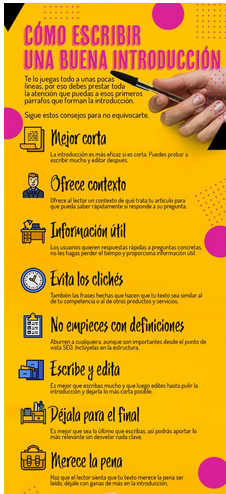
\includegraphics[scale = 0.95]{Figuras/intro.png}
	\end{center}
	\caption{\label{fig:recintro} Recomendaciones sobre la introducción}
\end{figure}






 \chapter{Apartados del CUERPO DEL DOCUMENTO}

El llamado ``cuerpo del documento'' es el grupo de apartados donde se describe como  se ha desarrollado el trabajo. En el dominio de la Informática, un TFG debe mantener un equilibrio entre la componente de investigación y la componente puramente técnica asociada con el proyecto de desarrollo de software. Un projecto software conlleva la elaboración de una serie de memorias, cada una recopilando lo hecho a distintos niveles, ver figura \ref{fig:report}. Sin embargo la memoria de un TFG es de carácter académico y ademas de artefactos, presupuestos y modelos debe incluir determinadas cuestiones que muestren como se han desarrollado las ideas propias. El punto de partida es la estructura típica de un articulo que se muestra en la figura \ref{fig:articulo}.


\begin{figure}

	\begin{center}
		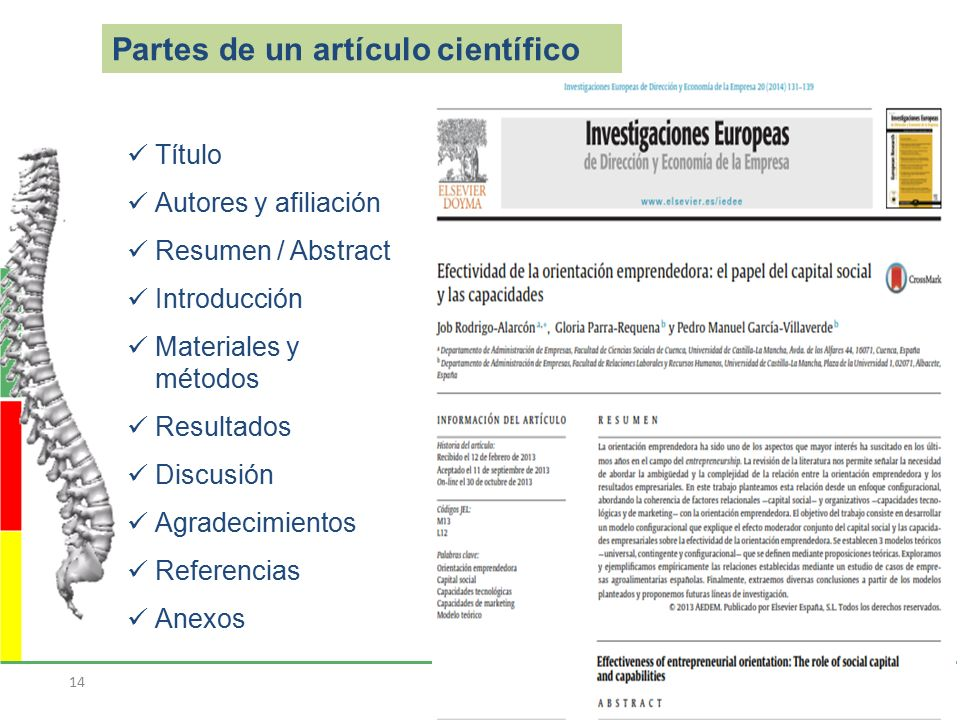
\includegraphics[scale = 0.45]{Figuras/articulo.jpg}
	\end{center}
	\caption{Estructura clásica de un articulo de investigación}
	\label{fig:articulo}
\end{figure}


\begin{figure}  
 	\begin{center}
        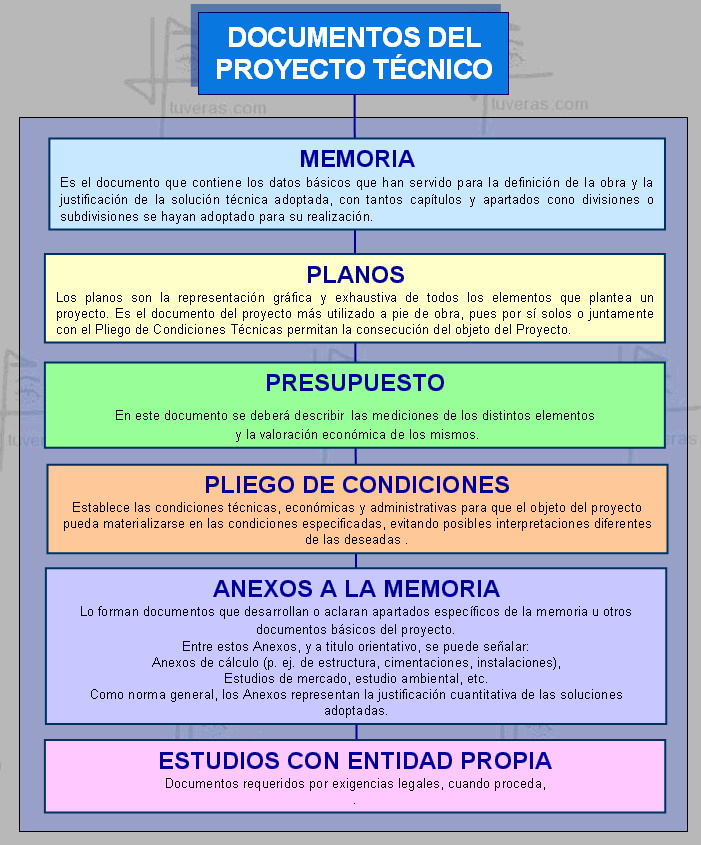
\includegraphics[scale = 0.45]{Figuras/documentos.jpg}
        	\end{center}
        \caption{Estructura de documentos de un proyecto técnico}
    \label{fig:report}
\end{figure}


La propuesta de estructura se define a continuación indicando que se incluiría en cada apartado. Lo importante en este caso es \textsc{que hay que incluir} la estructura del TFG final de cada alumno puede ser diferente, uniendo o separando los contenidos que se detallan a continuación. 

\paragraph{Objetivos o cuestiones de investigación}

se establecerá el objetivo general y los específicos, es decir, cuestiones que serán respondidas con el trabajo que se va a realizar. No es
imprescindible elaborar un apartado específico denominado OBJETIVOS, pues éstos puede quedar reflejados al final de la
introducción

\paragraph{Planificación temporal} 
Se debe incluir una referencia a como se han distribuido las tareas a lo largo del tiempo empleado en el TFG. Esta cuestión deriva de los proyectos técnicos de disciplinas de ingeniería. Puede representarse en forma de tabla o gráfico \ref{fig:plan} y puede aparecer dentro del apartado de metodología.



\begin{figure} 
\begin{ganttchart}[
hgrid,
vgrid={*6{draw=none},dotted},
x unit=0.5mm,
y unit title =0.6cm,
y unit  chart=1cm,
canvas/.style={draw=none},
%title/.append style={fill=black!10, rounded corners=1mm},
title/.append style={ rounded corners=0.5mm},
time slot format=isodate,
time slot format/base century=2000,
time slot unit= day,
time slot format/start date=2020-11-25,
bar height=0.5,
 bar label node/.append style={left=0.01cm, align=left, text width=8em},
 bar label text={$\star$#1},
 bar label font=\sffamily\footnotesize,
 group label node/.append style={left=0.01cm, align=left, text width=8em},
  group peaks width={3},
   group label font=\bfseries\footnotesize,
milestone label font=\scshape\sffamily\footnotesize,
  milestone inline label node/.append style={left=5mm},
  milestone right shift=2,
    milestone left shift=-2,
 milestone/.append style={fill=black!40}
]{2020-11-24}{2021-06-30}
\gantttitlecalendar[y unit title=0.7cm, title height=0.6]{year, month=shortname ,week} \\

\ganttgroup[ bar height=.1]{Selección área}{2020-11-24}{2020-11-30} \\
\ganttbar[name=b2]{Envío de Correos de contacto}{2020-11-24}{2020-11-26}\\
\ganttbar[name=b2]{Realizar Entrevistas}{2020-11-27}{2020-11-30}\\
\ganttmilestone{Área y tutor definido}{2020-11-30} \\ %\ganttnewline
\ganttgroup[bar height=.1]{Estudio preliminar}{2020-12-01}{2020-12-22}\\
\ganttlinkedbar{Task 2}{2020-12-01}{2020-12-22} \\
\ganttbar{Final Task}{2020-12-01}{2020-12-22}\\
\ganttbar{Task 2}{2020-12-01}{2020-12-22}
%\ganttlink{elem2}{elem3}
%\ganttlink{elem3}{elem4}
\end{ganttchart}
        \caption{Planificación del proyecto sobre latex}
    \label{fig:planb}
\end{figure}


\begin{figure}  
 	\begin{center}
        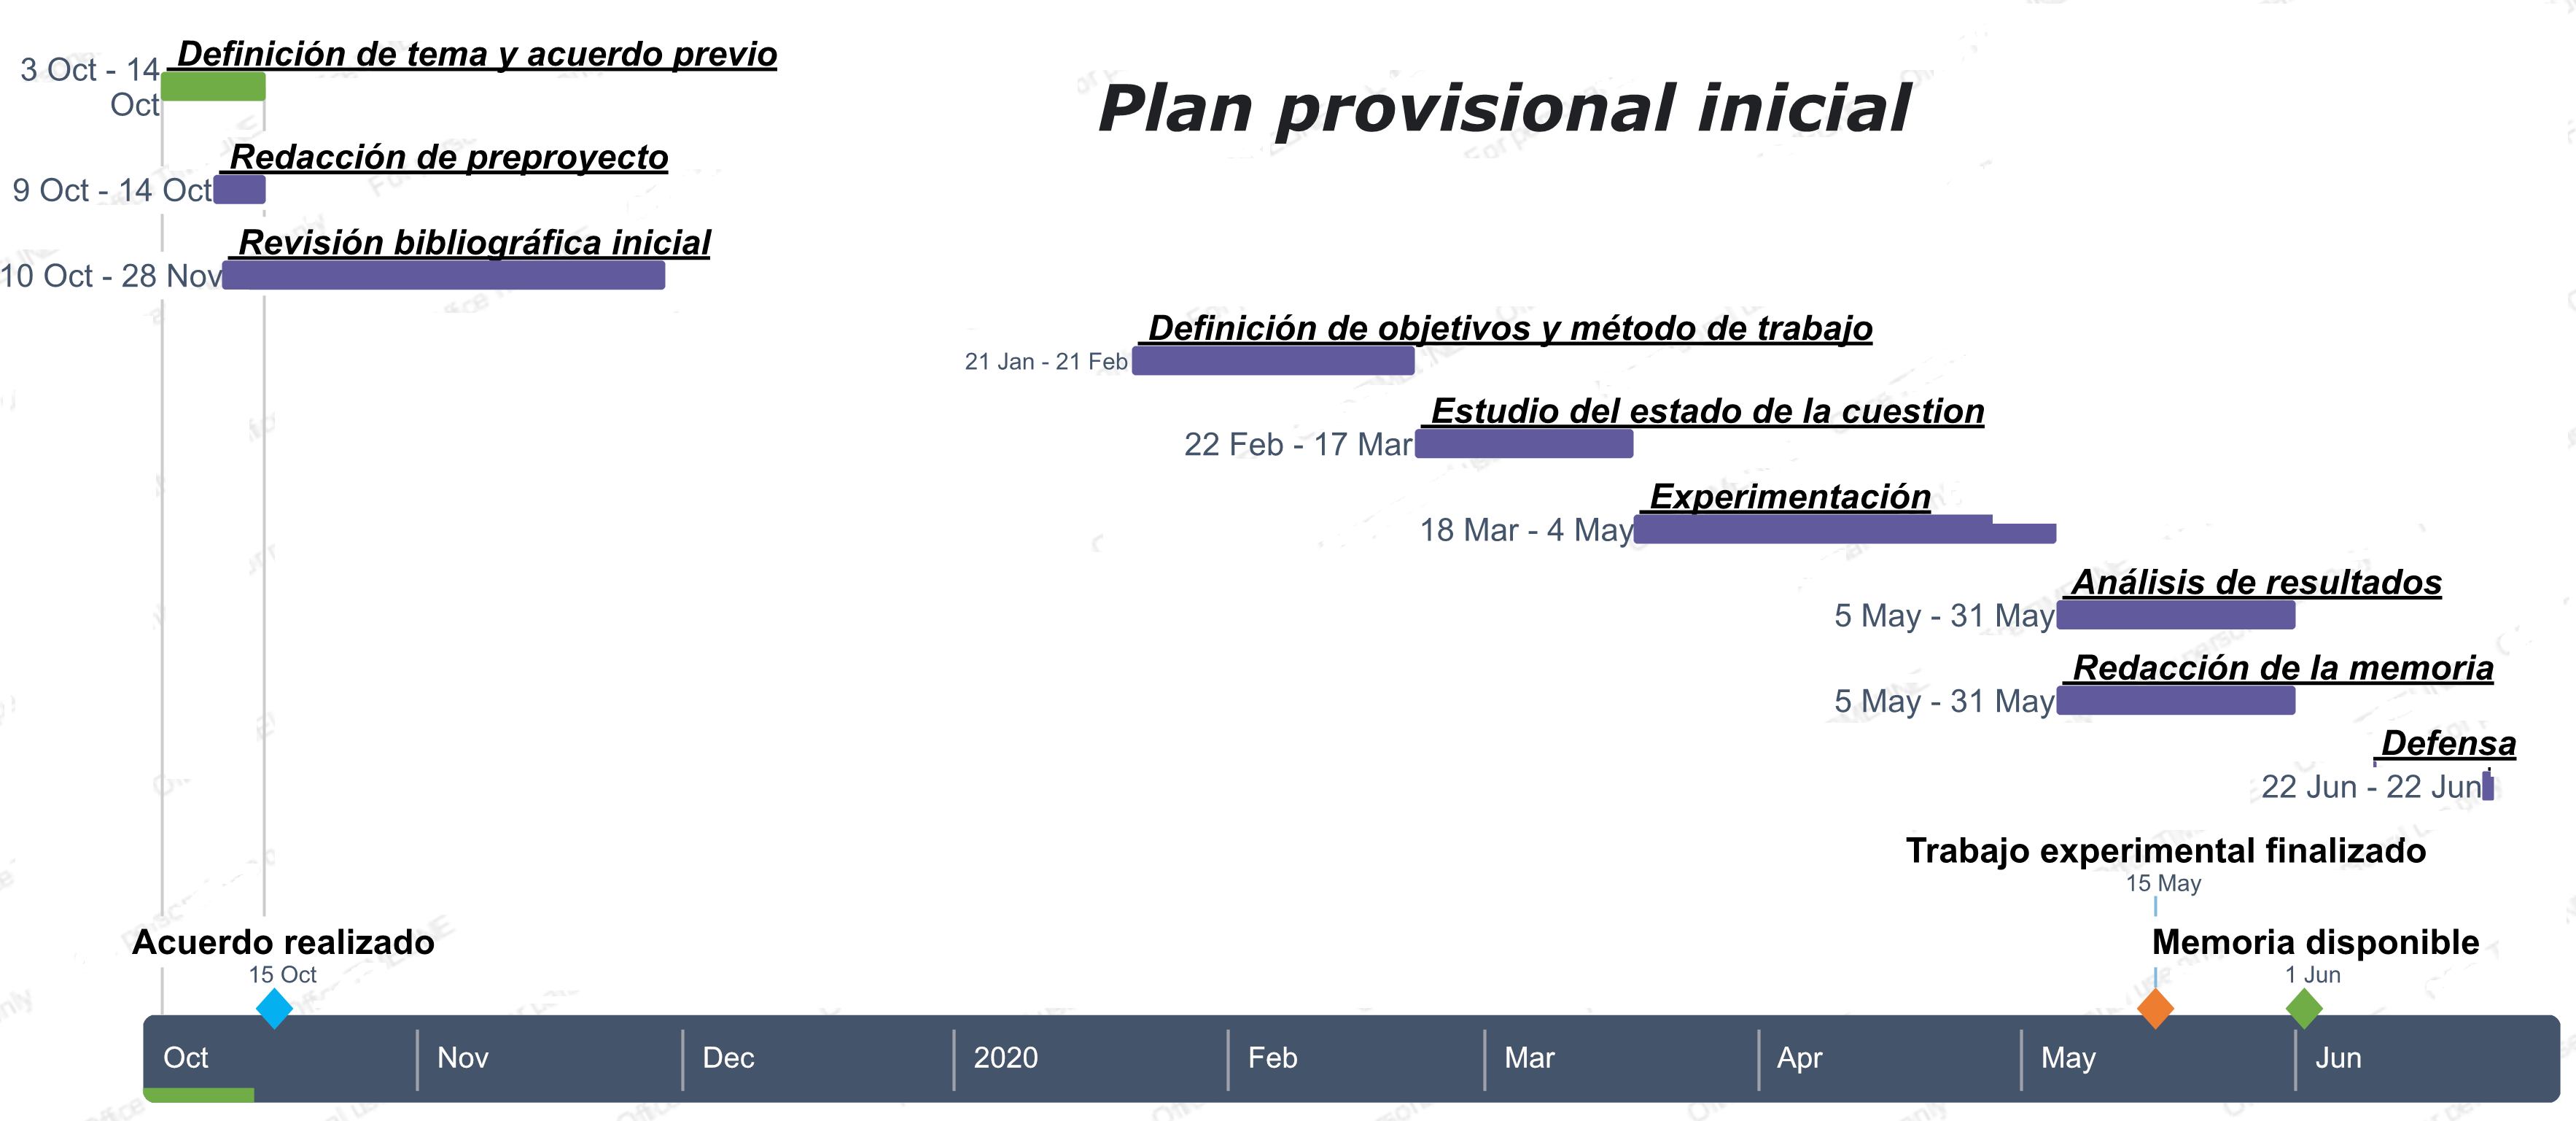
\includegraphics[width=0.8\textwidth]{Figuras/plandef.png}
        	\end{center}
        \caption{Planificación del proyecto}
    \label{fig:plan}
\end{figure}

\paragraph{Contextualización o estado del arte}

Se hará mención a los elementos conceptuales que  sirven  de  base  para  la  investigación,  estudios  previos  relacionados  con  el problema planteado, etc. En este apartado es importante hacer un estudio de los trabajos previos o revisión bibliográfica \cite{kitchenham2009systematic,kitchenham_2013}. Si como es habitual se tiene  que utilizar una o varias herramientas software es en este apartado donde se recogen las alternativas consideradas y cual de ellas ha sido elegida  y porqué.

\paragraph{Metodología}
¿Qué procedimiento se ha seguido para alcanzar los objetivos
planteados? Se  indicará  el  tipo  o  tipos  de  investigación,  las  técnicas  y  los procedimientos  que  serán  utilizados  para  llevarla  a  cabo;  se  identificará la población  y  el  tamaño  de  la  muestra  así  como  las técnicas  e  instrumentos  de recolección de datos, si te trata de un trabajo empírico, la metodología de desarrollo de software seleccionada. O cualquier otra información sobre el proceso seguido. La planificación y objetivos también pueden estar en este apartado

 
\paragraph{Resultados}
Incluirá  los  resultados  de  la  investigación  o  trabajo,  así como el análisis y la discusión de los mismos, aunque algunos tutores prefieren dos apartados separados. En el caso de tratarse de un desarrollo de software en este apartado se incluirá la descripción del producto resultante y los modelos o artefactos softtware necesarios para su descripción. Pero el manual o tutorial detallado  y los modelos completos deberían llevarse a los anexos.


La discusión conlleva revisar que aporta el trabajo realizado y se  han conseguido los objetivos planteados inicialmente. Caso de tener una evaluación por parte de los clientes potenciales también aparecerá en este apartado.


 \chapter{Apartado BIBLIOGRAFIA}
 Este apartado es de vital importancia para tener éxito en la consecución del trabajo fin de grado. Los tribunales suelen prestar gran atención a este apartado, probablemente por su formación académica. 
 
 Es todo un mundo el de los estilos bibliográficos y la realización de las citas, se puede encontrar un tutorial en:  \url{http://ci2.ual.es/comunicar-la-informacion/citas-y-referencias-bibliograficas/}. No obstante en las siguientes secciones se indicarán las cuestiones básicas para iniciarse en el tema pero restringuiendose a la utilización de la presente plantilla. La gran ventaja de latex es que cada elemento en las referencias   \lstinline[language=enparrafo]!\bibitem! es considerado como un elemento de una base de datos, de forma que es el compilador el que reordena o coloca la cita de acuerdo con el estilo definido.

 \section{Como citar}
A lo largo del texto de la memoria se incluirán citas a trabajos de otros autores. La inclusión de la cita tiene que ser justo después del texto donde se propone algo relativo al trabajo citado. Para citar, como para todo el \LaTeX{} existen numerosos paquetes, los dos mas conocidos son  biblatex y   natbib . 

Además dada forma de citar y de incorporar items en el apartado referencias lleva asociado un estilo de bibliografía    \lstinline[language=enparrafo]!\bibliographystyle{XXX}!, que aun abre mucho mas el abanico de opciones. 

Es recomendable consultar las ayudas de los paquetes \url{https://www.overleaf.com/learn/latex/Biblatex_bibliography_styles} y \url{https://www.overleaf.com/learn/latex/Bibliography_management_with_natbib}.

Lo habitual es utilizar la orden      \lstinline[language=enparrafo]!\cite{xxx}!, o   \lstinline[language=enparrafo]!\citep(xxx)!  en la ubicación en el texto donde se quiere colocar la cita, el compilador se encargá de procesarla según el estilo.

 \section {Apartado referencias}
  Existen dos formas de incorporar las referencias, directamente en el entorno   \lstinline[language=enparrafo]!\begin{bibliography}! y utilizando las ordenes del lenguaje o bien utilizando un archivo .bib para guardar esas referencias. Se generará un auxiliar .bbl que automáticamente se incorpora en el documento.
  
  Este archivo auxiliar es el que tiene directamente las ordenes del lenguaje.
  
 \begin{verbatim}
  
\begin{thebibliography}{3}

\bibitem{SWEBOK2014}
P.~Bourque and R.~E. Fairley, Eds., \emph{{SWEBOK}: Guide to the Software
  Engineering Body of Knowledge}, version 3.0~ed.\hskip 1em plus 0.5em minus
  0.4em\relax Los Alamitos, CA: IEEE Computer Society, 2014.

\bibitem{kitchenham_2013}
B.~Kitchenham and P.~Brereton, ``A systematic review of systematic review
  process research in software engineering,'' \emph{Information and Software
  Technology}, vol.~55, no.~12, pp. 2049 -- 2075, 2013.

\bibitem{basili1992}
V.~R. Basili, ``Software modeling and measurement: the goal/question/metric
  paradigm. cs-tr-2956, umiacs-tr-92-96,'' University of Maryland, Tech. Rep.,
  1992.
\end{thebibliography}

  \end{verbatim}
 
 
 
 \section{Archivos .bib}
 
 BibTeX, y natbib por extensión, usan un archivo externo en texto plano como base de datos de referencias bibliográficas para generar las bibliografías y sus referencias en documentos con distintos formatos de artículos, libros, tesis, presentaciones, etc. Los nombres de archivos de referencias bibliográficas de BibTeX usualmente terminan o usan la extensión .bib. Los ítems bibliográficos incluidos en un .bib están separados por tipos.
 
 \begin{verbatim}
@inbook{Berander2005,
        address = {Berlin, Heidelberg},
        author = {Berander, Patrik and Andrews, Anneliese},
        booktitle = {Engineering and Managing Software Requirements},
        pages = {69--94},
        publisher = {Springer Berlin Heidelberg},
        title = {{Requirements Prioritization}},
        doi= {https://doi.org/10.1007/3-540-28244-0{\_}4},
        year = {2005}
} 
 \end{verbatim}
 
 Los tipos que son reconocidos por virtualmente todos los estilos de BibTeX se muestran en el anexo \ref{sec:bib}. Pero igual que antes es recomendable recurrir a tutoriales o recursos donde se describan con detalle. Además se recomienda la utilización de algún gestor de referencias bibliográficas tipo Mendeley. \url{https://www.mendeley.com/}
 
 %%Capturas con nombre de pie de pagina
 \newfloat{Captura}{thp}[numerador]
 
 \flimage{Equipo}{Miembros Equipo}
 \flimage{osadia}{Faccion Equipo}



\addcontentsline{toc}{section}{BIBLIOGRAFÍA}
\bibliography{referencias}

\appendix
%\clearpage


\addtocontents{toc}{ \vspace{5mm} \hrule \par}


\chapter {Contenido de una entrada en .bib}
\begin{table} 
	\begin{center}
	\begin{tabular}{l p{10cm} }
		\textbf{Nombre campo} & \textbf{Descripción} \\ \hline

address&Usualmente la dirección de la editorial\\
author&Nombre(s) del (de los) autor(es)\\
title&Título del libro\\
chapter&El número de un capítulo (o sección, etc)\\
edition&La edición de un libro, por ejemplo,segunda\\
editor&Nombre(s) del (de los) editor(es)\\
howpublished&Forma en que fue publicada la obra\\
institution&Institución responsable de un informe técnico\\
journal&Nombre del periódico o revista\\
key&Empleado para la alfabetización, referencias cruzadas y para crear una clave cuando la información del autor no está disponible. No debe confundirse con la etiqueta usada en el cite y que debe colocarse al inicio de la entrada\\
month&El mes de publicación o, para un trabajo inédito, en el que fue escrito\\
note&Cualquier información adicional que pueda ayudar al lector\\
number&El número del periódico, la revista, el informe técnico o del trabajo en una serie\\
organization&La organización responsable de una conferencia o que publica un manual\\
pages&Números de páginas\\
publisher&El nombre de la editorial. No debe confundirse con el editor\\
school&Nombre de la escuela donde fue escrita una tesis\\
series&El nombre de una serie o conjunto de libros\\
title&El título del trabajo\\
type&El tipo de un informe técnico\\
volume&El volumen de un periódico o una revista, o de algún libro que conste de volúmenes\\
year&El año de publicación. Para un trabajo inédito, el año en que fue escrito. Generalmente debe consistir de cuatro dígitos, por ejemplo 200\\
         \hline
	\end{tabular}
	\end{center}
	\caption{Campos de una entrada en archivo de bibliografía .bib}
\end{table}



  \chapter{Tipos de referencias}
  \label{sec:bib}
    \begin{table} 
	\begin{center}
	\begin{tabular}{l p{10cm} }
	 \hline
   article& Un artículo de un periódico o revista\\
  
    book& Un libro con una editorial que se indica en forma explícita. Los campos requeridos en este caso son author (autor), editor, title (título), publisher (editorial) y year (año)\\
  
    booklet& Una obra que está impresa y encuadernada, pero sin una editorial o institución patrocinadora\\
  
    conference& Lo mismo que inproceedings, incluido para compatibilidad con el lenguaje de marcación Scribe\\
  
    inbook& Una parte de un libro, que puede ser un capítulo (o sección) o un rango de páginas\\
  
    incollection& Una parte de un libro que tiene su propio título\\
  
    inproceedings& Un artículo en las actas de sesiones (proceedings) de una conferencia\\
  
    manual& Documentación técnica\\
  
    mastersthesis& Una tesis de maestría (Master thesis) o proyecto fin de carrera\\
  
    misc& Para uso cuando los demás tipos no corresponden\\
  
    phdthesis& Una tesis de doctorado (Ph D thesis)\\
  
    proceedings& Las actas de sesiones de una conferencia\\
  
    techreport& Un reporte publicado por una escuela u otra institución, usualmente numerado dentro de una serie\\
  
    unpublished& Un documento que tiene un autor y título, pero que no fue formalmente publicado\\
          \hline
	\end{tabular}
	\end{center}
	\caption{Tipos posibles de elementos en bibligrafía con natbib}
\end{table}

 
  \chapter *{Artefactos software}




%\input{pmbok}

\clearpage
\backmatter

\thispagestyle{empty}
%\put(0,0){
\begin{minipage}[h]{0.9\paperwidth}
\thispagestyle{empty}
\begin{tikzpicture}[remember picture,overlay]
\node (f) [rectangle]  
at (current page.center)
          {\parbox[b][\paperheight]{\paperwidth}{
           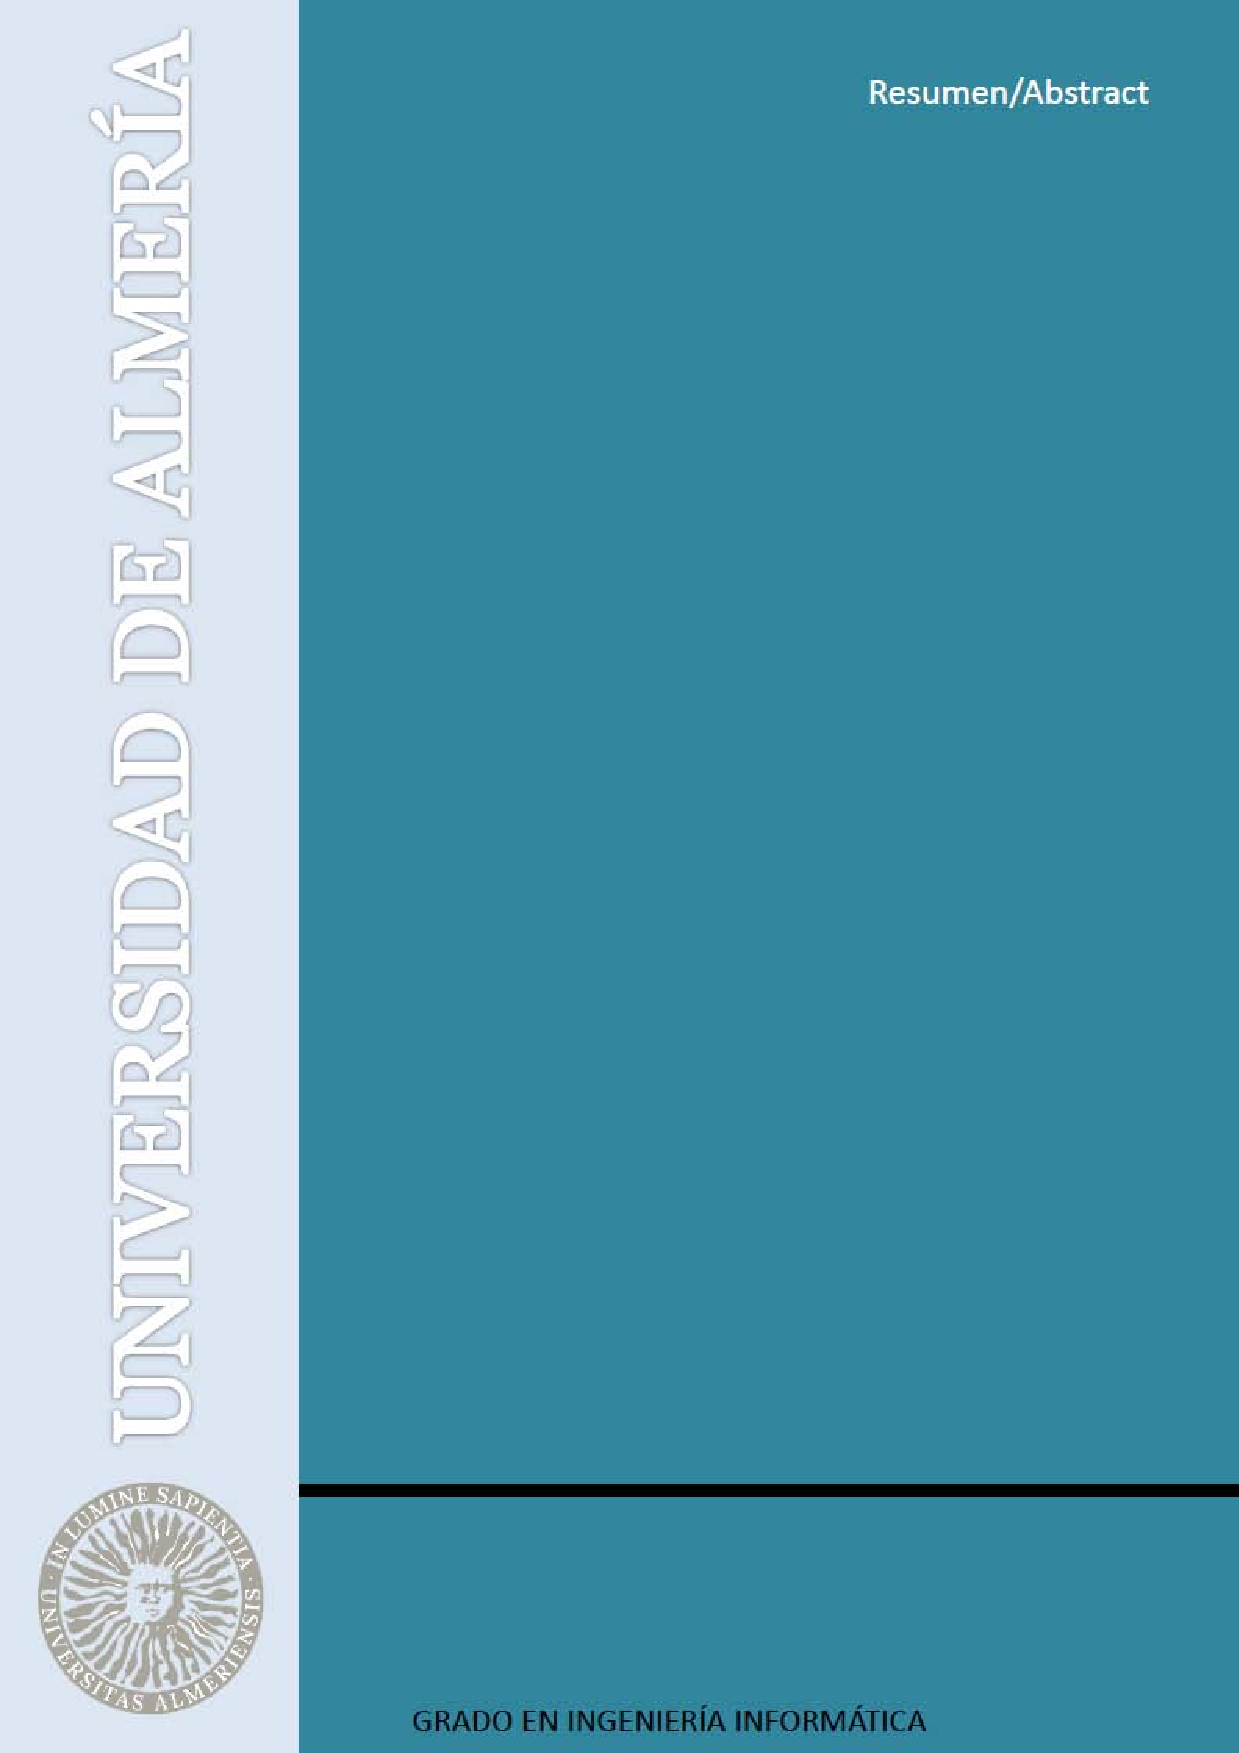
\includegraphics[width=\paperwidth,height=\paperheight,keepaspectratio]{Figuras/logos/TFG_back}
          }};
\node (texto) [rectangle,text width=0.5\paperwidth,yshift=150pt] 
at (f)
          {\parbox{0.65\paperwidth}{\justifying \Large \color{white}
         En este archivo se incluirá tanto el resumen en castellano como su traducción al inglés. Los dos párrafos estarán ligeramente separados.

El  propósito  del  trabajo  en  una  o  dos  frases.  El  diseño  y metodología  utilizada,  los  resultados  más  significativos  del trabajo realizado y un breve resumen de las conclusiones. Debe ser conciso y presentar los resultados obtenidos tras la ejecución del TFG. 

\vspace{1.5cm}

%\section*{Abstract}
Put here  the english tranlation  ... . Debe ser conciso y presentar los resultados obtenidos tras la ejecución del TFG. Los dos parrafos estarán ligeramente separados.
         }};
       \node  at (14,-25.55) {\Large\curso};
  \end{tikzpicture}
\end{minipage}
%}


          
          

\end{document}

